\section{What is a Netlist?}
\label{sec:netlist}
In its most general form, a netlist is a list of every component in an electronic design paired with a list of nets they connect to. 
Depending on the working abstraction level, these components can be transistors, logic gates, macrocells, or increasingly higher-level modules. 
Generally, a net denotes any group of two or more interconnected components.
In an electronics context, a net can be though of as a wire connecting multiple pins between multiple components, with each wire having one voltage source and one or more voltage sinks. 
Thus, one could express the netlist as a hypergraph, nodes representing component ports, hyperedges representing wires connecting two or more component ports. 
More precisely, these hyperedges connect the pins between the components, not the components themselves, with each component exposing multiple pins or ports. 

In FPGA context, the components are logical cells (\texttt{LUTs}, \texttt{CARRY4s}, etc.) or hierarchical cells (Verilog module instances) with pins connected together by wires. 
In Vivado, a Netlist can be synthesized as a Hierarchical or a Flattened netlist. 
Figure ~\ref{fig:hierarchical_design} shows an example a Verilog design using module instance hierarchy, while figure ~\ref{fig:hier_netlist} shows the design synthesized into a hierarchical netlist with \textbf{hierarchical cells} and \textbf{leaf cells}. 
The synthesizer attempts to construct the module hierarchy as close to the module instantiation hierarchy defined by the user design entry. 
Figure ~\ref{fig:flat_netlist} shows the same design but synthesized into a flattened netlist. 

In either synthesized netlist, the \textbf{leaf cells}, (deepest level cells), must necessarily consist only of \textbf{primitive cells} from the architecture's primitive cell library (\texttt{LUT6}, \texttt{FDRE}, \texttt{CARRY4}, \texttt{DSP48E1}, etc.). 
The netlist can be compiled and exported as a purely structural low-level Verilog file, or an Electrinic Design Interchange Format (EDIF) file, both describing the netlist explicitly as a list of logical cells connected by a list of wires. 

\end{multicols}
{
    \raggedright
    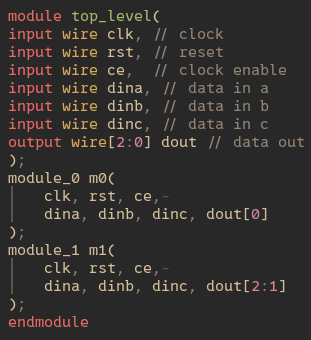
\includegraphics[valign=t, scale=0.3]{figures/netlist_synth/top_level.png}
    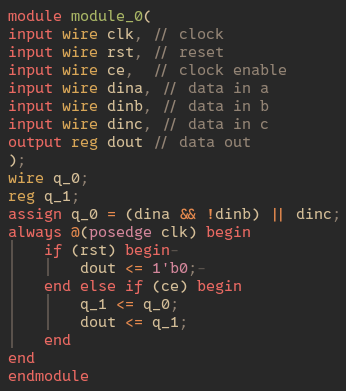
\includegraphics[valign=t, scale=0.3]{figures/netlist_synth/module_0.png}
    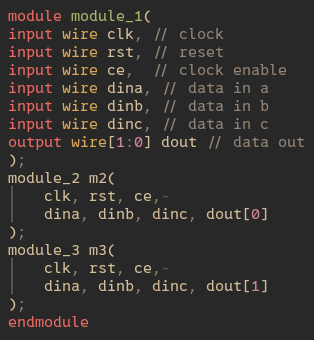
\includegraphics[valign=t, scale=0.3]{figures/netlist_synth/module_1.png}
    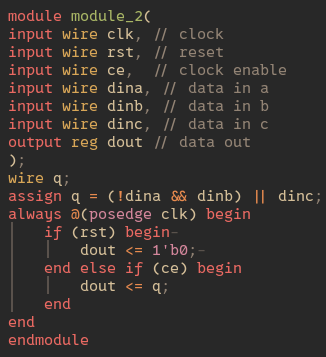
\includegraphics[valign=t, scale=0.3]{figures/netlist_synth/module_2.png}
    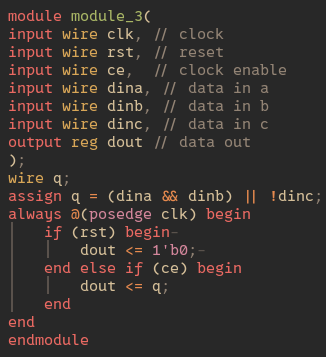
\includegraphics[valign=t, scale=0.3]{figures/netlist_synth/module_3.png}
    \captionof{figure}{A simple HDL design with module hierarchy.}
    \label{fig:hierarchical_design}
}
{
    \centering
    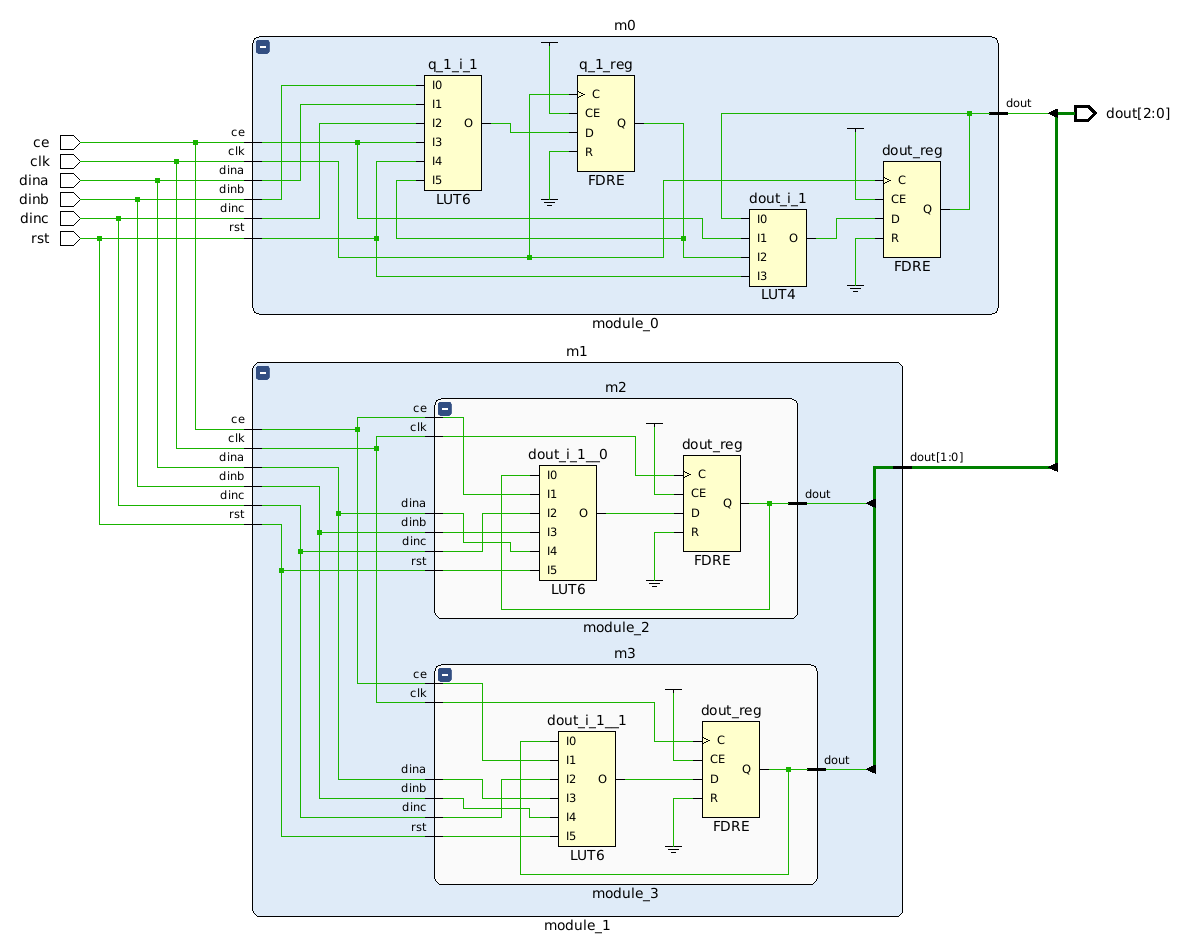
\includegraphics[valign=c, width=11.5cm]{figures/netlist_synth/hier_netlist.png}
    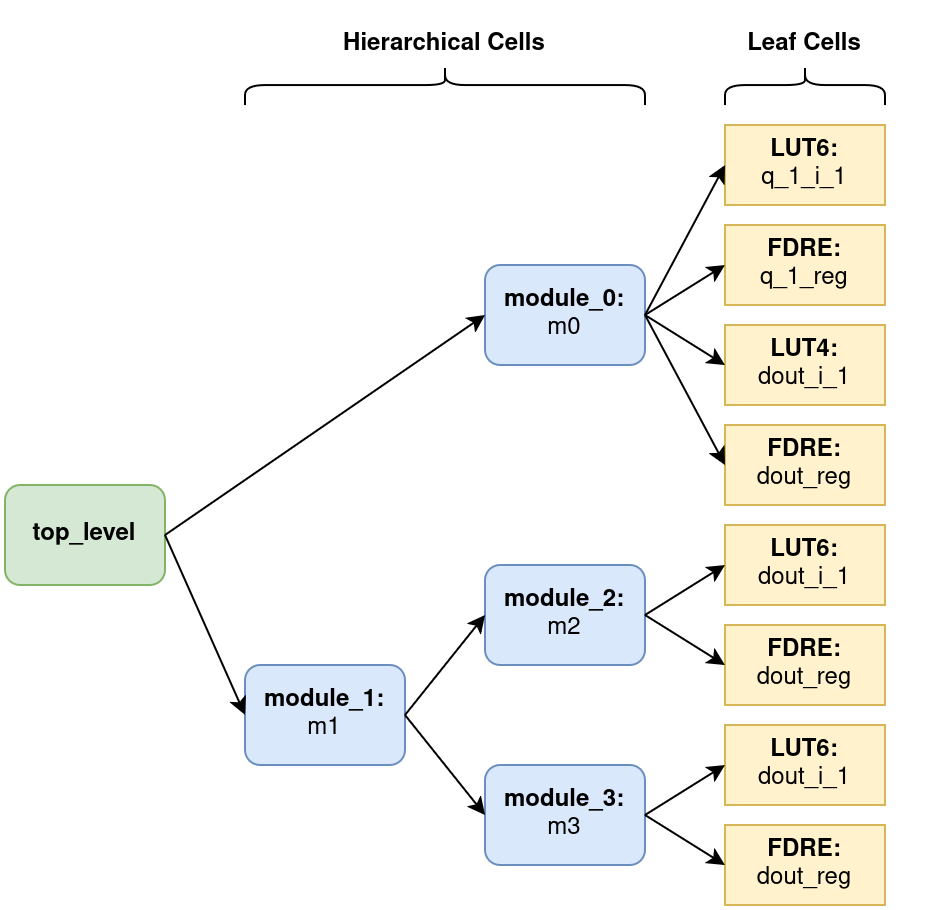
\includegraphics[valign=c, width=6cm]{figures/netlist_synth/hier_graph.png}
    \captionof{figure}{
        \textbf{Left:} A hierarchical netlist consisting of LUTs and FFs.
        \textbf{Right:} The cell hierarchy graph.
    }
    \label{fig:hier_netlist}
}
\vspace{0.5cm}
{
    \centering
    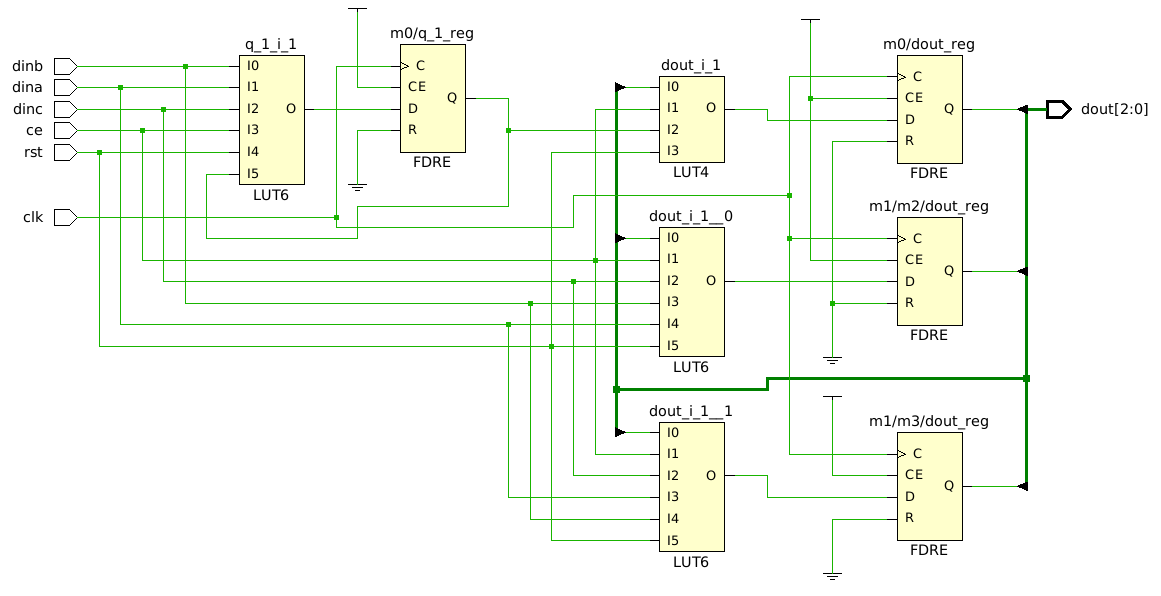
\includegraphics[valign=c, width=13cm]{figures/netlist_synth/flat_netlist.png}
    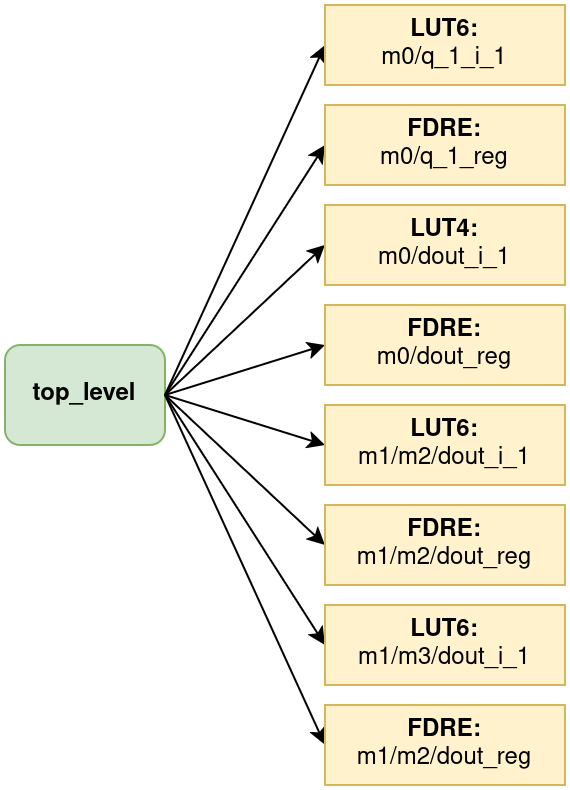
\includegraphics[valign=c, width=4cm]{figures/netlist_synth/flat_graph.png}
    \captionof{figure}{
        \textbf{Left:} A flattened netlist consisting of LUTs and FFs.
        \textbf{Right:} The flattened cell hierarchy graph.
    }
    \label{fig:flat_netlist}
}
\begin{multicols}{2}

\subsection{Netlist Traversal and Manipulation in RapidWright}

\begin{itemize}
\item


\end{itemize}

One of RapidWright's most powerful features is netlist traversal and manipulation via the \texttt{edif} classes. A netlist can be easily extracted from a \texttt{.dcp} design checkpoint and traversed like the following: 

\begin{lstlisting}[language=java, caption={Netlist extraction and traversal}, label={lst:netlist_extract}]
Design design = Design.readCheckpoint("synth.dcp")
EDIFNetlist = design.getNetlist();

// Example task:
// Extract the set of all unique nets from the design.

// Initialize a new Set:
Set<EDIFNet> netSet = new HashSet<>();

// Access all leaf cells
List<EDIFCellInst> ecis = netlist.getAllLeafCellInstances();

// Traverse the cell list
for (EDIFCellInst eci : ecis) {
    // Access the ports on this cell
    Collection<EDIFPortInst> epis = eci.getPortInsts();
    for (EDIFPortInst epi : epis) {
        // Access the net on this port
        EDIFNet net = epi.getNet();
        netSet.add(net);
    }
}

// Downstream task:
// For each unique net, print out the connected cells.

// Traverse the set of nets
for (EDIFNet net : netSet) {
    System.out.println("Net: " + net.getName());
    // Access the ports connected to this net
    Collection<EDIFPortInst> epis = net.getPortInsts();
    for (EDIFPortInst epi : epis) {
        // Access the cell that this port belongs to
        EDIFCellInst eci = epi.getCellInst();
        if (eci == null) {
            // (top_level ports have no associated cell)
            continue;
        } else {
            System.out.println(
                "\tCell: " + eci.getName() + 
                ",\tCellType: " + eci.getCellName()
            );
        }
    }
}

\end{lstlisting}


{
    \centering
    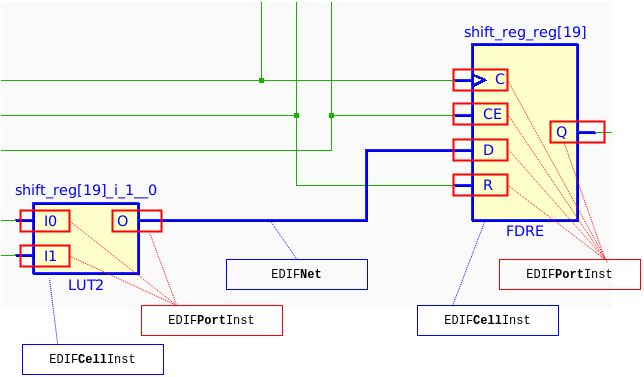
\includegraphics[valign=c, width=\columnwidth]{figures/traversal.png}
    \captionof{figure}{\textttt{Netlist} traversal via \texttt{EDIFHierCellInst}, \texttt{EDIFHierPortInst}, and \texttt{EDIFHierNet} objects}
    \label{fig:traversal}
}


